\chapter{Literature Review}
\section{Introduction}
In this chapter, each of the elements of the work flow outlined in this project are discussed with relation to work published in similar areas. The areas of particular focus are data pre-processing, unsupervised learning and supervised learning. Each section will outline and explain certain concepts covered in this thesis and also look at papers with similar challenges.
\lhead{\emph{Background}}
\section{Data Pre-processing}
Data pre-processing is the work done to transform a data-set prior to applying any machine learning algorithms. On a basic level, different algorithms require different structures to the data in order to compile. An example of this is some algorithms handling missing data poorly so often the data points with missing values are investigated and either removed or imputed. There are many other potential roadblocks that can prevent an algorithm from working such as correct date formatting, there are also another set of operations which transform the existing data in order to increase the performance of the model. For instance removing outliers, normalizing the data set or accounting for seasonal difference will all help towards improving the accuracy of the model. Depending on the data set and the aim of the model, the steps taken in the data pre-processing can vary. Models that work with word processing will have to tokenize the words and count the frequency, some data sets containing variables such as gender or colour are transformed into dummy variables which represent categorical variables as binary variables.

\\


\section{Unsupervised Learning}
\subsection{Clustering}
Clustering is a solution for classifying and labelling data into distinct classes when there is no prior knowledge about the existence of these classes, this is referred to as unsupervised classification. This project will analyse energy consumption data of domestic consumers measured on a 30 minute time resolution over the period of 2 years. The initial goal is to partition the consumers based on habitual behaviour in order to develop energy consumption profiles, the role of clustering becomes clear. \\
Clustering is the process of taking $n$ number of data points and fitting them to $j$ number of disjointed clusters. In this scenario, all data points within an individual cluster are similar however each cluster is distinct from any other. There are numerous techniques used for unsupervised clustering, one of which is $k$-means clustering, favoured by virtue of being one of the more straight forward techniques available ~\cite{KMC}. $k$-means clustering finds the partition of the data given $n$ number of observations into $k (\leq n)$ sets $S = \{S_1,S_2, \dots, S_k\}$ so as to minimize the within-cluster sum of squares. This can be represented as the following:

\begin{equation}
\stackrel{arg min}{_{S}} \sum_{i=1}^k \sum_{x \epsilon S_{i}} \Vert x-\mu_{i} \Vert ^{2} = \stackrel{arg min}{_{S}}  |S_{i}|  Var S_{i}
\end{equation}
Where $\mu_{i}$ is the mean of points in $S_i$. This is equivalent to minimizing the pairwise squared deviations of points in the same cluster:
\begin{equation}
\stackrel{arg min}{_{S}} \sum_{i=1}^k \frac{1}{2|S_i|} \sum_{x, y\epsilon S_i}\Vert x- y \Vert ^2
\end{equation}
A limitation of the $k$-means is that it is only optimal for spherical clusters. The clusters are to be expected to be of equal or similar size which may not always be the case. There are other models available such as the Gaussian models which are more flexible by having both variances and covariances.

One common method used to predict or monitor future values for time series data is classification methods which assign a category to patterns in the series. 

\subsection{Hierarchical Clustering}
Similarity or dissimilarity is a method by which a data set can be partitioned based on the distance between static objects . There are different distance measurements designed for specifying similarity between time-series. Hausdorff distance, modified Hausdorff (MODDH) HMM-based distance, Euclidean distance, Euclidean distance in a PCA subspace, and Longest Common Sub Sequence (LCSS) are the most popular distance measurement methods that are used for time-series data \cite{AGHABOZORGI201516}.\\
In building energy profiles, for balanced general solutions, Euclidean distance is the measure that obtains the best results. Dynamic Time Warping (DTW) distance can be regarded as an improved alternative distance measurement over Euclidean distance in applications that make the most of better representation of the high-similar nuclei and where losing capabilities to capture and average the no-so-similar samples is not a critical factor ~\cite{8581840920130201}.\\

\subsection{Distance Measurement MPdist}
As mentioned above, Euclidean Distance and Dynamic Time Warp (DTW) have been accepted into the community as two effective measurement distances but these measures are not without fault as we can see in ~\cite{Gharghabi2018AnUT}. Shaghayegh et al. introduces a new measure called MPdist, the advantage of this measurement is being able to handle missing values or spurious regions. Additionally using this measurement over the Euclidean or DTW measures increases computation efficiency. In the field of energy consumption where a huge amount of data is continually generated, this is advantages as it allows for analysis on larger quantities of data streams. Some necessary definitions must be outlined before defining the MPdist formula as found in ~\cite{Gharghabi2018AnUT}.\\


\textbf{Definition 1:} A Time Series T = $t_1, t_2, \dots, t_n$ is a sequence of $n$ real values. MPdist is a distance measurement between two time series.\\
\textbf{Definition 2:} A subsequence T$_{i,L}$ is a contiguous subset of values with length $L$ starting from position $i$ in the time series T. The subsequence T$_{i,L}$ is in the form T$_{i,L} = t_i, t_{i+1},\dots, t_{i+L-1}$ where $1 \leq L \leq |T|$\\
\textbf{Definition 3:} Sliding window. All possible subsequences of a given time series T can be extracted by sliding a window of size $L$ across T. There are ($n - L + 1$) such subsequences, which we denote as $SubseqNum$.\\
At a high level, the proposed MPdist measurement will compute the distance between two time series T$_A$ and T$_B$, by aggregating the distances between All-subsequences set. For this purpose, we need to find the nearest neighbor for each subsequence in A within B (and visa versa). To determine if a member of set B is the nearest neighbor of a member in set A we use 1NN-Join Function.\\
\textbf{Definition 4:} An All-Subsequences Set A is a set of all possible subsequences of a time series T. The subsequences are obtained from sliding a window of length $L$ across T. Thus,\\
\begin{equation}
A = \{T_{1,L}, T_{2,L},\dots, T_{n-L+1,L}\}
\end{equation}\\
\textbf{Definition 5:} 1NN-Join Function is defined as the first nearest neighbor (1NN) between two subsequences A[$i$] and B[$j$].\\
The 1NN-join function is a similarity join operator, which is applied on two All-subsequence sets, as a result we can create the AB similarity set:\\
\textbf{Definition 6:} AB Similarity Join J$_{AB}$ is a set containing pairs of each subsequence in A with its corresponding nearest neighbor in B. In which A and B are two sets of All-subsequences. $J_{AB}$ is defined as:
\begin{equation}
J_{AB} = \{\langle A[i], B[j]\rangle \; | \; \theta_{1NN}(A[i], B[j])\}
\end{equation}\\
The similarity join set contains tuples, with each subsequence in a set A from the time series T$_A$, and its nearest neighbor in set B from time series T$_B$. Note that some subsequences in T$_B$ may not be used as neighbors to any elements from T$_A$, and some subsequences in T$_B$ may be used more than once. This is because in general $J_{AB} \neq J_{BA}$.\\
For the proposed MPdist distance measure, we need to obtain the distance between each pair in the similarity join set. After obtaining the nearest neighbor of each subsequence in a set, an array which stores the Euclidean distance of each pair is called the Matrix Profile.\\
\textbf{Definition 7:} Matrix Profile P$_{AB}$ is an array in which the Euclidean distance between each pair in $J_{AB}$ is stored. The length of $P_{AB}$ is ($n - L + 1$) or $SubseqNum$. \\
Without loss of generality, it is assumed that the two time series T$_A$ and T$_B$ have the same length. Moreover, it rarely makes sense to measure the similarity of time series with significantly different lengths.\\
Fig. 2.1 shows the $P_{AB}$ of two time series T$_A$ and T$_B$. As shown, since T$_A$ and T$_B$ have most common structure, their P$_AB$ has low values except for the region where sine-waves change to triangular wave, in which case there is no "explanation" from T$_{B}$ in T$_{A}$, hence, there is a bump in P$_{AB}$ indicating a high value.

\begin{figure}
\centering     
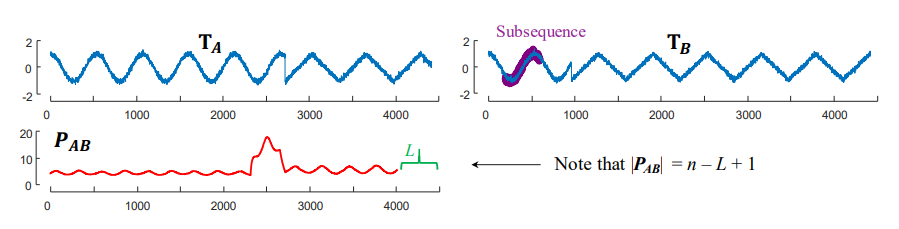
\includegraphics[width=1\textwidth]{Figures/MPdist_fig3.png}
\caption{(top) Two time series T$_A$ and T$_B$, (bottom) P$_{AB}$ of two time series T$_A$ and T$_B$ with $L = 400$. Because there is no corresponding section in T$_A$ from T$_B$ at the point of signal change, there is a bump in P$_{AB}$}
\label{fig:MPdist}
\end{figure} 

The time complexity to calculate P$_{AB}$ for two equal-length time series with $L$ is much shorter than $n$ is $O(n^2)$. If the length of $L$ is a significant fraction of $n$, then the time complexity grows to $O((n - L + 1) \times n)$. In the limit, when $L = n$, this degenerates to the special case of Euclidean distance between two time series, which takes $O(n)$. The following notation summarizes this:

\begin{equation}
\textrm{Time complexity } P_{AB} = \Bigg\{ \substack{
O(n^2)\ \\
O((n - L + 1) \times n), \\
O(n),
}
\substack{
L \ll n \\
L < n \\
L = n}
\end{equation}

As $L$ approaches $n$, the time complexity approaches linear time. To make this distance measure between T$_A$ and T$_B$ symmetric, both J$_{AB}$ and J$_{BA}$ need to be computed. This is denoted as the ABBA similarity join:

\textbf{Definition 8: } ABBA Similarity Join J$_{ABBA}$ is a set containing pairs of subsequence in A with its nearest neighbor in B and vice versa.\\
Note that if a subsequence in A (denoted as T$_{A,i}$) is the nearest neighbor of a subsequence in B (denoted as T$_{B,j}$) the reverse of that may not be true. An array which stores all distances in ABBA similarity join set is Join Matrix Profile:
\\
\textbf{Definition 9: }Join Matrix Profile P$_{ABBA}$ is an array contain the Euclidean distance for each pair in J$_{ABBA}$. The length of the P$_{ABBA}$ is $2 \times (n - L) + 2$ which is twice the length of P$_{AB}$.
\\
The  matrix profile has distances for both similarity joins J$_{AB}$ and J$_{BA}$, thus it is symmetric in terms of the order of the time series. As a result, the distance calculated based on J$_{ABBA}$ between T$_{A}$ and T$_{B}$ is also equal. Fig. 2.2 shows an illustration of the P$_{ABBA}$ of two time series T$_{A}$ and T$_{B}$.

\begin{figure}
\centering     
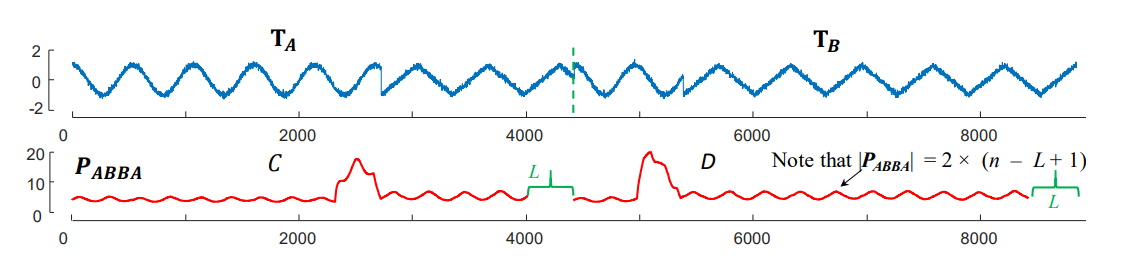
\includegraphics[width=1\textwidth]{Figures/MPdist_fig4.png}
\caption{(top) The concatenation of two time series T$_A$ and T$_B$, (bottom) P$_{ABBA}$ of two time series T$_A$ and T$_B$ with $L = 400$. The distance between each subsequence from T$_A$ and its nearest neighbor from T$_B$ is calculated in C and the reverse in D. There is a gap between C and D at the middle, because the length of the remaining data in T$_A$ is less than the subsequence length thus, the distance cannot be calculated.}
\label{fig:MPdist}
\end{figure} 

The MPdist formula is as follows:

\begin{equation}
MPdist = \Bigg\{ 
\stackrel 
    {k^{th} \textrm{value of sorted} P_{ABBA}}
    {max(P_{ABBA}),}
\qquad 
\stackrel
    {|P_{ABBA}| > k}
    {|P_{ABBA}| \leq k}
\end{equation}

The worse case complexity of MPdist is $O(n^2)$ which would make it unsuitable for large datasets.However as shown in ~\cite{Gharghabi2018AnUT}, the complexity can be reduced to $O(m \times SubseqNum)$ time.



\subsection{Fuzzy Logic}
There is scope here to introduce fuzzy logic, as  Maharaj et al. outline ~\cite{MAHARAJ20111187}, fuzzy logic allows a non-strict representation of object membership to a set. These membership grades indicate the degree to which the data points belong to each cluster. In conventional clustering techniques data points right on the boundary of a cluster hold the same relationship to the cluster as those in the very centre. Using the membership grade, these points at edge of the cluster can still be inside the cluster but to a lesser degree than those at its centre. This may be necessary due to imprecise and uncertain data introduced through for example, faulty monitoring equipment. Fuzzy k-means is a clustering method that has proved effective in many scenarios since it permits the assignment of data elements to one or more clusters ~\cite{MOLINASOLANA2017598}. Fuzzy logic is based on minimization of the following objective function:

\begin{equation}
J_m = \sum_{i=1}^{n} \sum_{j=1}^{c} u_{ij}^{m} \Vert x_i - c_j \Vert  \qquad  \textrm{for}   \quad i \leq m < \infty
\end{equation}

where, membership:
\begin{equation}
u_{ij} = \frac{1}{\sum_{k=1}^c (\frac{\Vert x_i - c_j \Vert}{\Vert x_i - c_k \Vert})^ \frac{2}{m-1}}
\end{equation}\\
cluster centres:
\begin{equation}
c_j = \frac{\sum_{i=1}^n u_{ij}^m . x_i}{\sum_{i=1}^n u_{ij}^m}
\end{equation}

%https://www-sciencedirect-com.cit.idm.oclc.org/science/article/pii/S0020025510005840 \\
%https://home.deib.polimi.it/matteucc/Clustering/tutorial_html/cmeans.html

Here, $m$ is the fuzzy parameter taking on any real number greater than 1. Values too close to 1 will result in a hard border like partition with all membership values close to 0 or 1. Large values of $m$ will result in homogeneous membership values close to $1/c$ ($c$ number of clusters). As such, neither values are used. In practice the most popular choice for the fuzzy parameter is $m = 2$, Hwang et al. chose $m = 2$ for their chosen model ~\cite{hwang}, as do Yang et al. in theirs ~\cite{4522596}. \\

% ADD THESE REFERENCES
%https://www-sciencedirect-com.cit.idm.oclc.org/science/article/pii/S0020025510005840\\
%https://link.springer.com/article/10.1007/s11336-005-1314-x \\
%https://books.google.ie/books?hl=en&lr=&id=z6XqBwAAQBAJ&oi=fnd&pg=PR14&ots=0h-OpWEnDr&sig=anHAa-7nUJzQURPcZcs4gABJUho&redir_esc=y#v=onepage&q&f=false \\ 
%https://ieeexplore.ieee.org/abstract/document/4522596 \\

Additionally, $u_{ij}$ is the degree of membership of $x_i$ in the cluster $j$ $x_i$ is the $i$th d-dimensional measured data, $c_j$ is the d-dimensional centre of the cluster, and $\Vert * \Vert$ is any norm expressing the similarity between any measured data and the centre.

% ADD THESE REFERENCES
%https://www-sciencedirect-com.cit.idm.oclc.org/science/article/pii/S0031320310003973